\begin{frame}[fragile]{Programs and Kernels}
  \begin{lstlisting}[gobble=4]
    prg = cl.Program(context, src)
  \end{lstlisting}
  \begin{columns}
    \column{0.65\textwidth}
      \begin{itemize}
        \item \texttt{src}: OpenCL device code
          \begin{itemize}
            \item Derivative of C99
            \item Functions with \texttt{\_\_kernel} attribute
              can be invoked from host
          \end{itemize}
        \item \texttt{prg.build(options="",\\
          \hspace*{2em}devices=None)}
        \item \texttt{kernel = prg.kernel\_name}
        \item \texttt{kernel(queue,\\
          \hspace*{2em}$(G_x,G_y,G_z)$, $(L_x,L_y,L_z)$, \\
          \hspace*{2em}arg, \dots, \\
          \hspace*{2em}wait\_for=None)}\\
      \end{itemize}
    \column{0.3\textwidth}
      % boo yuck
      \hspace*{-1cm}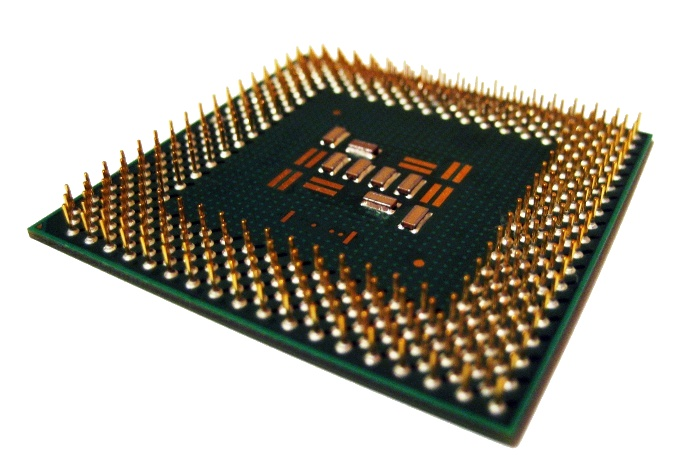
\includegraphics[width=1.3\textwidth]{cpu.jpeg}
  \end{columns}
\end{frame}
\begin{frame}[fragile]{Program Objects}
  \begin{lstlisting}[gobble=4]
    kernel(queue, (Gx,Gy,Gz), (Sx,Sy,Sz), arg, ..., wait_for=None)
  \end{lstlisting}
  \begin{columns}
    \column{0.3\textwidth}
      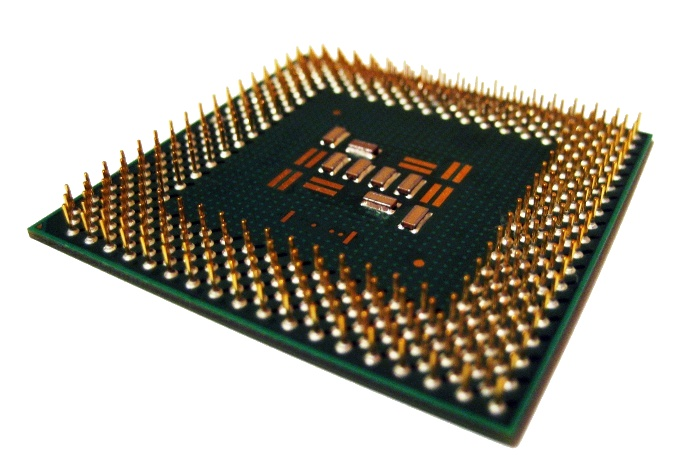
\includegraphics[width=1.3\textwidth]{cpu.jpeg}
    \column{0.65\textwidth}
      \begin{overlayarea}{\textwidth}{0.5\textheight}
        \only<+>{
          \texttt{arg} may be:
          \begin{itemize}
            \item \texttt{None} (a \texttt{NULL} pointer)
            \item \texttt{numpy} sized scalars:
              \texttt{numpy.int64,numpy.float32,\dots}
            \item Anything with buffer interface:\\
              \texttt{numpy.ndarray}, \texttt{str}\\
            \item Buffer Objects
            \item Also: \texttt{cl.Image}, \texttt{cl.Sampler}, 
              \texttt{cl.LocalMemory}
          \end{itemize}
        }
        \only<+>{
          Explicitly sized scalars:\\
          {\color{red}\ding{54}  Annoying, error-prone.}

          \medskip
          Better:

          \texttt{%
          kernel.set\_scalar\_arg\_dtypes([\\
          \hspace*{3ex}numpy.int32, None,\\
          \hspace*{3ex}numpy.float32])}
          \medskip

          Use \texttt{None} for non-scalars.
        }
      \end{overlayarea}
  \end{columns}
\end{frame}
\addimgcredit{CPU: sxc.hu/dimshik}
